% https://tex.stackexchange.com/questions/461161/drawing-a-circle-through-3-non-collinear-points
\documentclass[tikz,border=3mm]{standalone}
\usetikzlibrary{angles,through,calc,intersections}
\tikzset{
    circle through 3 points/.style n args={3}{% 
        insert path={
            let    
                \p1=($(#1)!0.5!(#2)$),
                \p2=($(#1)!0.5!(#3)$),
                \p3=($(#1)!0.5!(#2)!1!-90:(#2)$),
                \p4=($(#1)!0.5!(#3)!1!90:(#3)$),
                \p5=(intersection of \p1--\p3 and \p2--\p4)
            in },
        at={(\p5)},
        circle through= {(#1)}
    }
}

\begin{document}
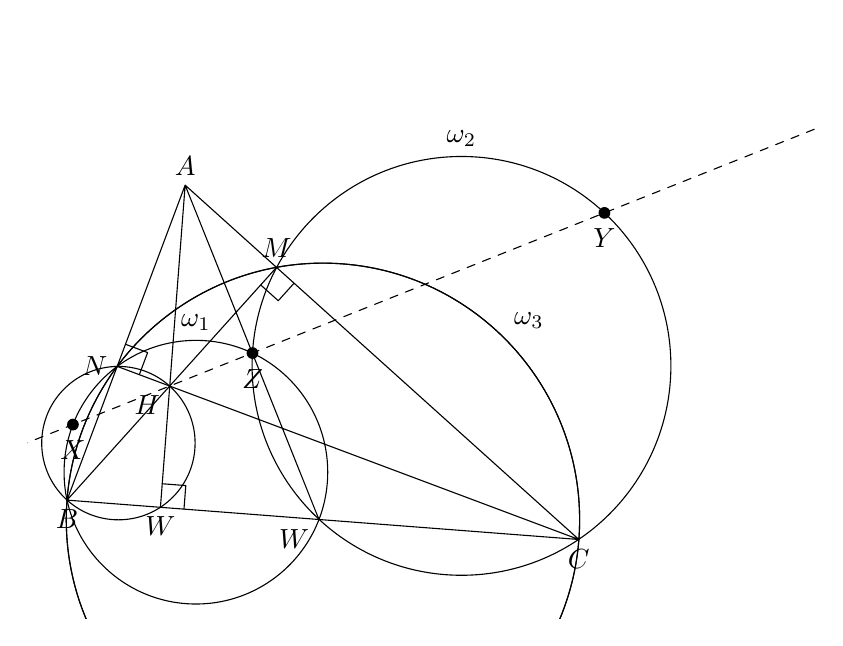
\begin{tikzpicture}[angle radius=0.3cm,line cap=round,line join=round,
    dot/.style={circle,fill,inner sep=1.5pt}]
    \draw (0,0) coordinate[label=above:$A$] (A) --
        (-1.5,-4)  coordinate[label=below:$B$] (B) --
        (5,-4.5) coordinate[label=below:$C$] (C) --cycle
        (A) -- ($(C)!(A)!(B)$) coordinate[label=below:$W$] (L)
        pic [draw] {right angle = C--L--A}
        (B) -- ($(A)!(B)!(C)$) coordinate[label=above:$M$] (M)
        pic [draw] {right angle = C--M--B}
        (C) -- ($(B)!(C)!(A)$) coordinate[label=left:$N$] (N)
        pic [draw] {right angle = C--N--A}
        (intersection of A--L and B--M) 
            coordinate[label=below left:$H$](H)
        let \p1=($(C)-(A)$),\p2=($(L)-(A)$), \n1={atan2(\y2,\x2)+atan2(\y1,\x1)}
        in ($(A)+(\n1/2:5)$) coordinate (aux) 
        (A) --
        (intersection of A--aux and B--C) coordinate[label=below left:$W$] (W) ;
    \begin{scope}  
        \clip (-2,-5.5)     rectangle (8,2);
        \path[nodes=draw] 
            node[circle through 3 points={B}{L}{N}] (BLN){}
            node[circle through 3 points={B}{C}{M}] (BCM){}
            node[circle through 3 points={C}{B}{M},label=above right:$\omega_3$] (CBM){}
            node[circle through 3 points={C}{M}{W},label=above:$\omega_2$] (CMW){}
            node[circle through 3 points={B}{N}{W},label=above:$\omega_1$] (BNW){};
        \foreach \X in {BLN,BCM,CBM,CMW,BNW}
            {\path[name path global=\X] let \p1=(\X.center),\p2=(\X.east) in 
                (\p1) circle[radius=\x2-\x1];}
        \path  [name intersections={of=CMW and BNW,by={Z,aux}}] 
            (Z) coordinate[dot,label=below:$Z$] (Z);
        \path[overlay,draw,dashed,name path=HZ] let \p1=($(Z)-(H)$),\n1={atan2(\y1,\x1)} in
            ($(Z)+(\n1:10)$) --  ($(Z)-(\n1:10)$);
        \path  [name intersections={of=HZ and BNW,by={aux,X}}] 
            (X) coordinate[dot,label=below:$X$] (X);
        \path  [name intersections={of=HZ and CMW,by={Y,aux}}] 
            (Y) coordinate[dot,label=below:$Y$] (Y);
    \end{scope} 
\end{tikzpicture}
\end{document}